%%\documentclass{beamer}
%%\documentclass[handout,usenames,dvipsnames]{beamer}
\documentclass[usenames,dvipsnames]{beamer}
\usepackage[numbers,totalnumber,sidebarshades]{beamerthemeUppsala}

\usepackage[utf8]{inputenc}
\usepackage[T1]{fontenc}
\usepackage{xcolor}
\usepackage{import}
\usepackage{listings}
\usepackage{hyperref}

%%%%%% Bibliograpy as footnotes %%%%
\usepackage{graphicx}
\usepackage[giveninits=true]{biblatex}
%\bibliography{../1DL010-21}

\graphicspath{{imgs/}}

\usepackage{pgfpages}
%\setbeameroption{show notes on second screen}
\setbeamertemplate{note page}{\insertnote}

%%\setbeamercovered{transparent}

\usepackage{xspace}
\usepackage{stmaryrd}
\usepackage{comment}

\newcommand{\tc}{\textcolor}
\newcommand{\largeskip}{\vspace{1cm}}
\newcommand{\nat}{\ensuremath{\mathbb{N}}}
\newcommand{\ra}{\ensuremath{\rightarrow}}

\newcommand{\states}{\ensuremath{S}}
\newcommand{\sts}{\ensuremath{s}}
\newcommand{\inits}{\ensuremath{s_I}}
\newcommand{\isg}{\ensuremath{g}}
\newcommand{\actions}{\ensuremath{A}}
\newcommand{\actf}{\ensuremath{\mathsf{av}}}
\newcommand{\acta}{\ensuremath{a}}
\newcommand{\trf}{\ensuremath{\delta}}
\newcommand{\costf}{\ensuremath{c}}
\newcommand{\utilf}{\ensuremath{u}}

\newcommand{\players}{\ensuremath{P}}
\newcommand{\maxp}{\ensuremath{\text{\textsc{max}}}}
\newcommand{\minp}{\ensuremath{\text{\textsc{min}}}}

\newcommand{\pts}{\ensuremath{PTS}}
\newcommand{\gts}{\ensuremath{GTS}}

\newcommand{\bstates}{\ensuremath{Q}}
\newcommand{\stb}{\ensuremath{q}}
\newcommand{\isf}{\ensuremath{f}}

\newcommand{\set}[1]{\ensuremath{ \{ #1 \}}}
\newcommand{\ol}{\ensuremath{\overline}}

\newcommand{\turnf}{\ensuremath{t}}

%%\newcommand{\land}{\wedge}
%%\newcommand{\lor}{\wee}
\newcommand{\lra}{\leftrightarrow}
\newcommand{\propl}{\mathcal{L}_p}

\newcommand{\M}{\mathcal{M}}
\newcommand{\lang}{\mathcal{L}}
\newcommand{\sat}{\ensuremath{\mathsf{SAT}}\xspace}
\newcommand{\limp}{\ensuremath{\mathsf{LIMP}}\xspace}

\newcommand{\const}{\boldsymbol}
\newcommand{\terms}{\mathit{TM}}
\newcommand{\term}{t}
\newcommand{\atoms}{ATOM}
\newcommand{\forms}{FORM}
\newcommand{\fv}{FV}
\newcommand{\struct}{\mathcal{S}}
\newcommand{\dom}{\Delta}

\newcommand{\intf}{I}

\newcommand{\te}{\ensuremath{\bar{v}}}
\newcommand{\va}{\ensuremath{v}}

\newcommand{\quant}{\ensuremath{\mathcal{Q}}}

\newcommand{\reals}{\ensuremath{\mathbb{R}}}

\newcommand{\hsig}{\ensuremath{h_{sig}}}
\newcommand{\logl}{\ensuremath{L_{\ell \ell}}}

\newcommand{\vechsig}{\ensuremath{\bar{h}_{sig}}}


%%%%%%%%%%%% Fabio ML %%%%%%%%%%%%%%%%%%
\def\riga{\vskip 1\baselineskip \noindent}
\newcommand{\bi}{\begin{itemize}\setlength{\itemsep}{-0.1em}}
\newcommand{\ei}{\end{itemize}}
\newcommand{\be}{\begin{enumerate}}
\newcommand{\ee}{\end{enumerate}}
%%%%%%%%%%%%%%%%%%%%%%%%%%%%%%%%%%%



%%%%%%%%%%% FNN %%%%%%%%%%%%%%%%%%%%
\newcommand{\nnw}[2]{w^{(#1)}_{#2}}
\newcommand{\nnW}[1]{\pmb{W}^{(#1)}}
\newcommand{\nna}[2]{a^{(#1)}_{#2}}
\newcommand{\nnA}[1]{\pmb{a}^{(#1)}}
\newcommand{\nnz}[2]{z^{(#1)}_{#2}}
\newcommand{\nnZ}[1]{\pmb{z}^{(#1)}}
\newcommand{\nnh}{\pmb{h}}
\newcommand{\nndelta}[2]{\delta^{(#1)}_{#2}}
\newcommand{\nnDELTA}[2]{\Delta^{(#1)}_{#2}}
\newcommand{\nnDelta}[1]{\pmb{\delta}^{(#1)}}
\newcommand{\nnDDELTA}[1]{\pmb{\Delta}^{(#1)}}


%%%%%%%%%%%%%%%%%%%%%%%%%%%%%%%%%%






%%%%%%%%%%%%%%%%%%%%%%%%%%%%%%%%%%%%%%%%
\title{1DT109 - Accelerating systems with FPGAs}
\subtitle{Formal verification}

\author[R.\ De Masellis]{Riccardo De Masellis}
\date[]{\today}
\institute[uu.se]{Uppsala University}

\begin{document}

\begin{frame}[plain]
  \titlepage
\end{frame}
%%%%%%%%%%%%%%%%%%%%%%%%%%%%%%%%%%%%%%%
\section{Introduction}
\frame{
\setbeamercovered{transparent}
\tableofcontents[currentsection,
        currentsubsection,
        subsectionstyle=shaded]
}
%%%%%%%%%%%%%%%%%%%%%%%%%%%%%%%%%%%%%%%
\begin{frame}
\frametitle{Why verification?}

%Desiderata:
\begin{ntblock}
\centering
To have an hardware free of bugs
\end{ntblock}

\vfill \pause 

\begin{itemize}
  \item What is a bug?
  \item \pause How do you define ``correct behaviour?'' \newline (extensionally, intentionally?)
\end{itemize}

  \end{frame}
 
 %%%%%%%%%%%%%%%%%%%%%%%%%%%%%%%%%%%%%%%

\begin{frame}
  \frametitle{Specification using english}
  
  \begin{center}
  ``This playground is forbidden to who: is shorter than 130cm or younger than 8 years old, if alone; \pause or is shorter than 110cm or younger than 6 years old if accompanied''.	


\vfill \pause

\includegraphics[scale=.4]{fry?}
\end{center}
\end{frame}


%%%%%%%%%%%%%%%%%%%%%%%%%%%%%%%%%%%

\begin{frame}
  \frametitle{Example: formal verification of a counter}
  
  \begin{ntblock}
  \centering
  Implement a synchronous \texttt{counter} that counts up to 4 \\ with an \texttt{enable} signal.
  \end{ntblock}
  
  \pause \vfill
  
  Ambiguous!
  \begin{itemize}
  \item Does the \texttt{counter} start from zero?
  \item if \texttt{enable}=1 then next value is previous value +1, but
  \item if \texttt{enable} $\not=$ 1 ? Shall we reset? Or next value is equal to previous value?
  \end{itemize}
\end{frame}


%%%%%%%%%%%%%%%%%%%%%%%%%%%%%%%%%%%%%%%

\begin{frame}
  \frametitle{Why FORMAL verification}

(Un-formal) verification and testing are not exhaustive, in general:
\begin{itemize}
\item hand-written test benches;
\item constrained random simulations.	
\end{itemize}


\vfill \pause

\begin{ntblock}

\centering

Formal verification guarantees (more or less) absence of bugs, by:
\begin{itemize}
  \item having unambiguous properties/specifications;
  \item analyzing all possible system behaviours.
\end{itemize}


\end{ntblock}

\end{frame}

%%%%%%%%%%%%%%%%%%%%%%%
%%%%%%%%%%%%%%%%%%%%%%%%%


%%%%%%%%%%%%%%%%%%%%%%%%%%%%%%%%%%%%%%%%%%%%%%%%%%%%%

\begin{frame}
  \frametitle{Importance of HW verification}
  
\begin{itemize}
\item In certain cases, especially in Embedded Systems, we can have critical components;
  \item Fixing HW is more expensive than fixing SW (e.g., Intel's bug).
\end{itemize}

\vfill

Indeed, it was HW industry pushed the development of formal verification techniques, which is nowadays always used (for HW).

\vfill \pause

\vfill
\begin{alertblock}{Question} 
Is it possible to always guarantee that HW/SW is free of bugs (theoretically/practically)?
  \end{alertblock}
\end{frame}

%%%%%%%%%%%%%%%%%%%%%%%%%%%%%%%%%%%%%%%%

\begin{frame}[fragile]
  \frametitle{Digression: the halting problem}
  
  \begin{alertblock}{The halting problem (proved by A. Turing, 1936)}
  	There is \tc{red}{no} program $halt(\cdot, \cdot)$ such that given as input any program $P(\cdot)$ and any input $x$, $halt(R, x)$ returns $1$ is $R(x)$ terminates and $0$ otherwise.
  \end{alertblock}
  
  \vfill \pause
  
Proof intuition (informal) by contradiction.
 \begin{itemize}
  \item Suppose $halt$ exists.
  \item Take the following program:
 \begin{verbatim}
  def R(x):
   if halt(R, x) then loop forever;
 \end{verbatim}
\pause \item now, if halt(R) is true (meaning: R terminates), then R loops forever, \tc{red}{contradiction};
\item therefore hypothesis on existence of $halt$ is faulty.
\end{itemize}
\end{frame}
%%%%%%%%%%%%%%%%%%%%%%%%%%%%%%%%%%%%%%%%

\begin{frame}
  \frametitle{Halting problem: in practice}
  
  \centering
  All programs that runs on a machine have finite memory, therefore finite inputs, thus \tc{blue}{in principle} they could be formally verified.
  
  \pause \vfill
  
  Analyze extensively the behaviour of a program, where states are all possible combination for values of variables.
  
\end{frame}

%%%%%%%%%%%%%%%%%%%%%%%%%%%%%%%%%%%%%%%%%%%%%%%%%%%%%%%

\section{What is formal verification}
\frame{
\setbeamercovered{transparent}
\tableofcontents[currentsection,
        currentsubsection,
        subsectionstyle=shaded]
}
%%%%%%%%%%%%%%%%%%%%%%%%%%%%%%%%%%%%%%%

\begin{frame}
  \frametitle{What formal verification does}
  
  \centering
  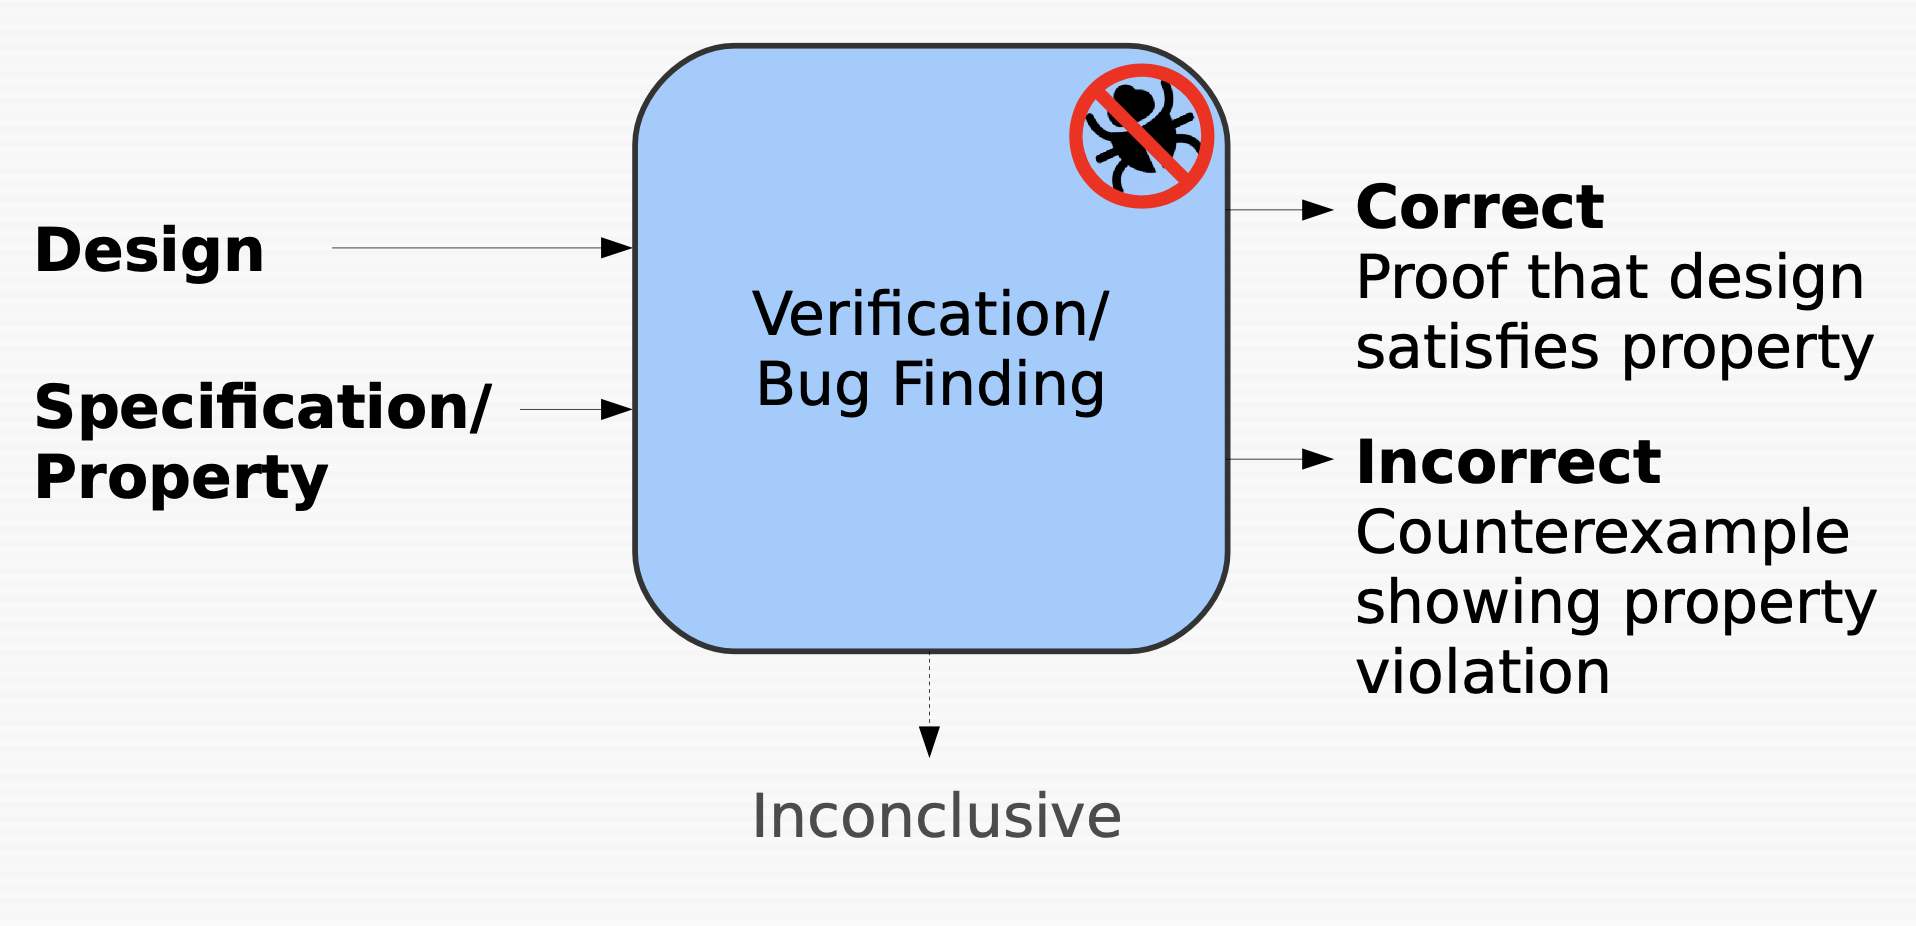
\includegraphics[scale=.3]{formal-verification}
  
  
\end{frame}
%%%%%%%%%%%%%%%%%%%%%%%%%%%%%%%%%%%%%%%

\begin{frame}
  \frametitle{Some techniques}
  
  \centering
  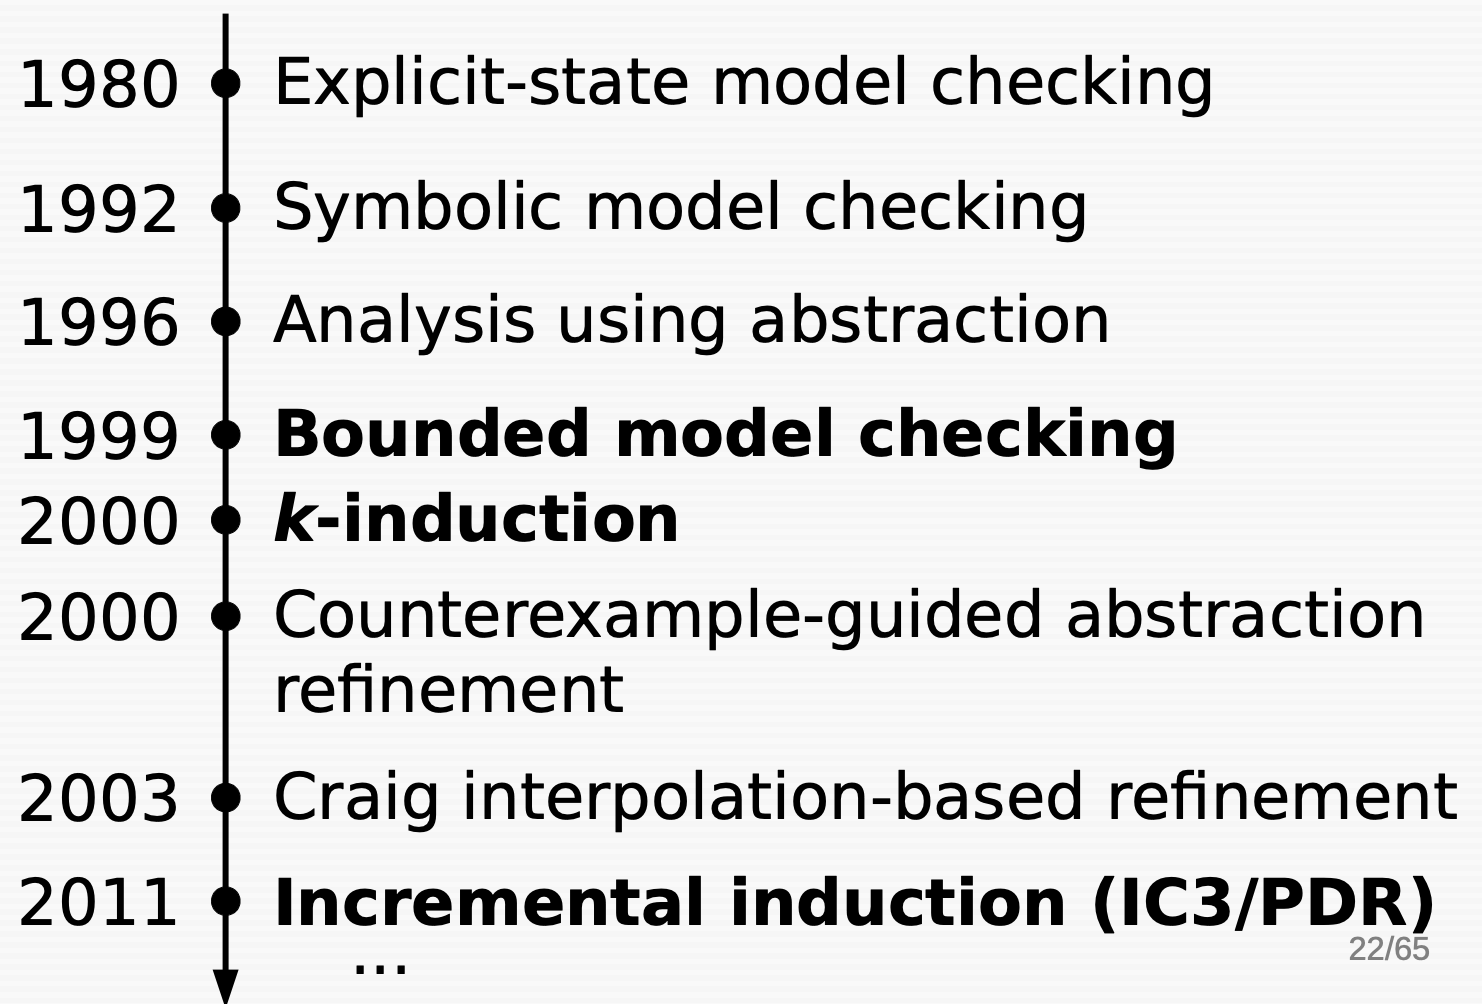
\includegraphics[scale=.35]{timeline}
  
\end{frame}

%%%%%%%%%%%%%%%%%%%%%%%%%%%%%%%%%%%%%%%

\begin{frame}[fragile]
  \frametitle{Explicit model checking, example}
  
\begin{lstlisting}[language=Verilog]
module counter(
  output [1:0] out, input enable, input clk);

  reg [1:0] count;
  assign out = count;

  initial count = 0;

  always @(posedge clk)
    if(enable)
     count = count + 1;
endmodule
 
 \end{lstlisting}

\end{frame}

%%%%%%%%%%%%%%%%%%%%%%%%%%%%%%%%%%%%%%%

\begin{frame}
  \frametitle{Explicit model checking, example cont'd}
  
  \centering
  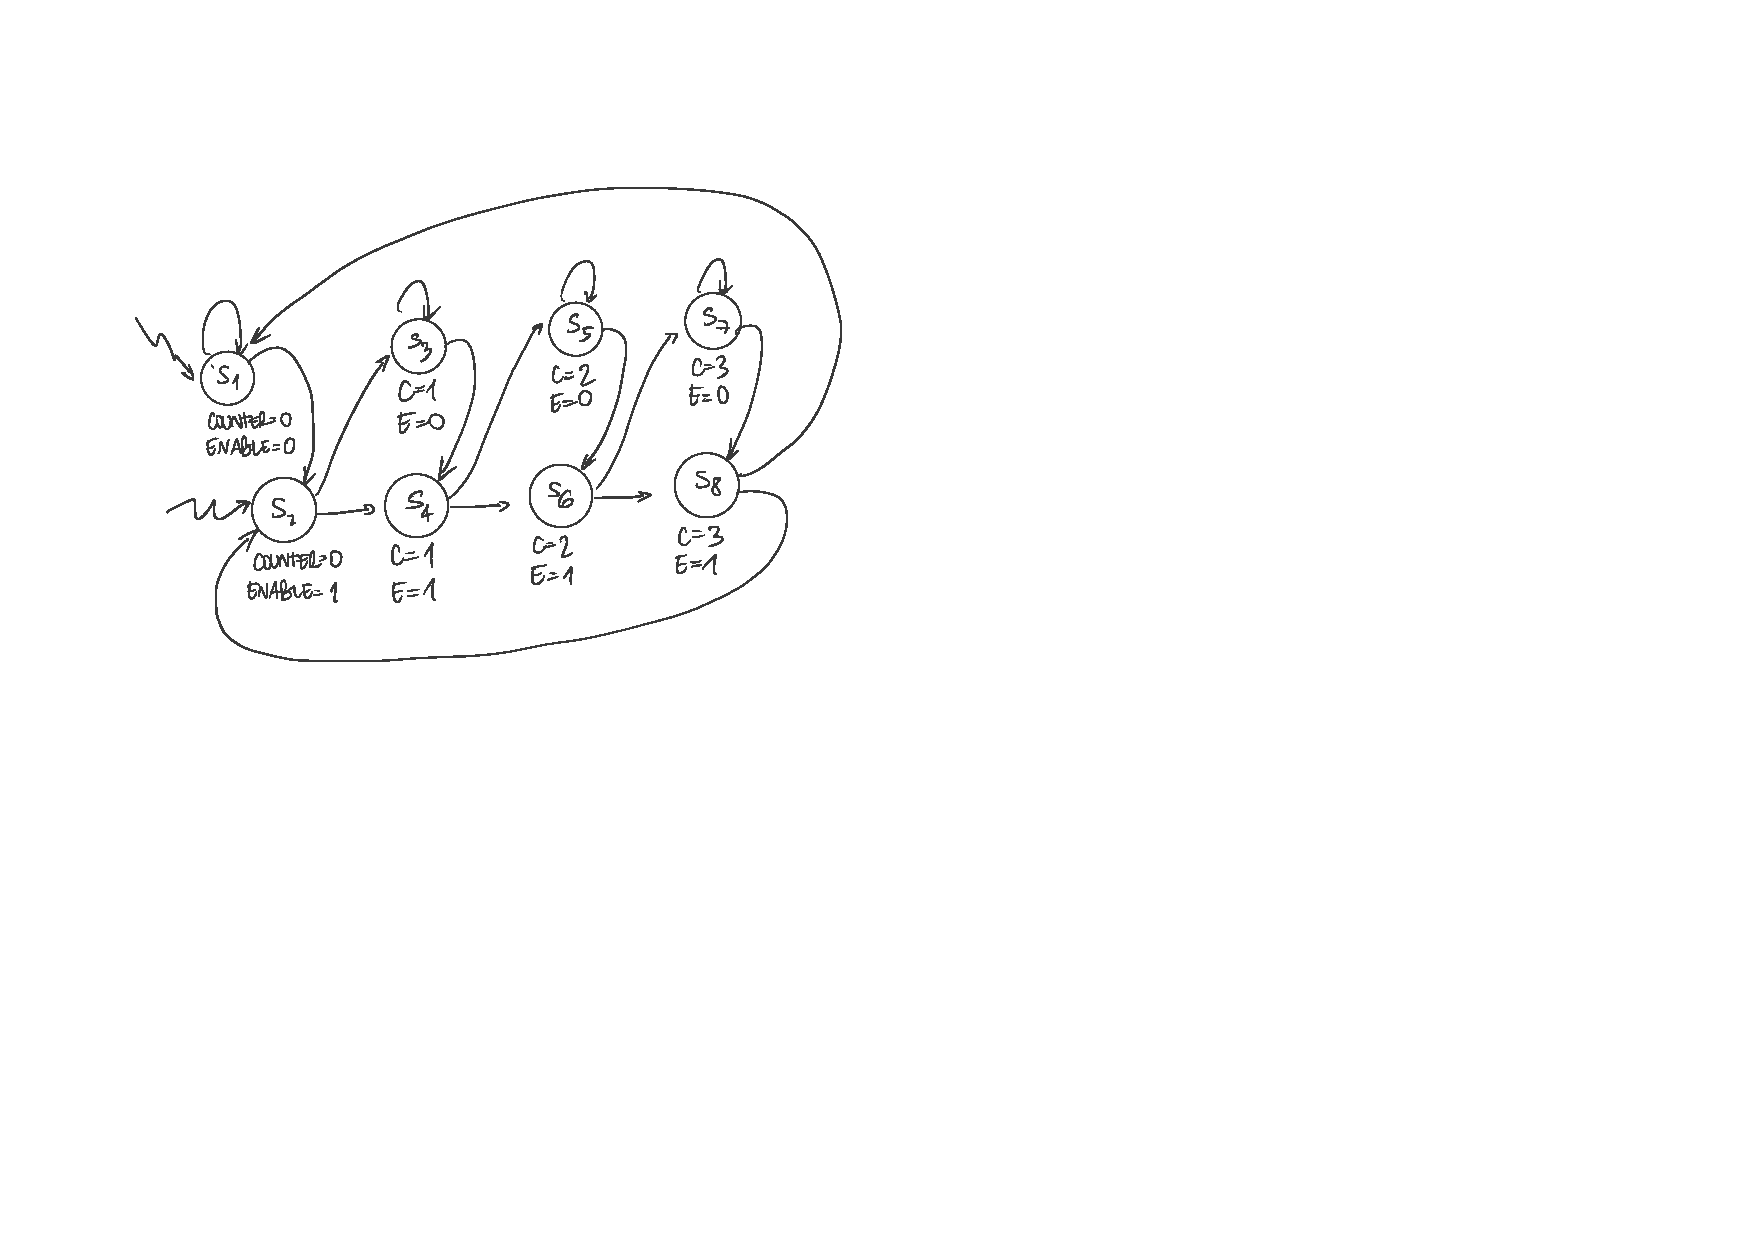
\includegraphics[scale=.7]{fsm}
  
\end{frame}

%%%%%%%%%%%%%%%%%%%%%%%%%%%%%%%%%%%%%%%

\begin{frame}
  \frametitle{Bounded model checking, example, cont'd}
  
  \centering
  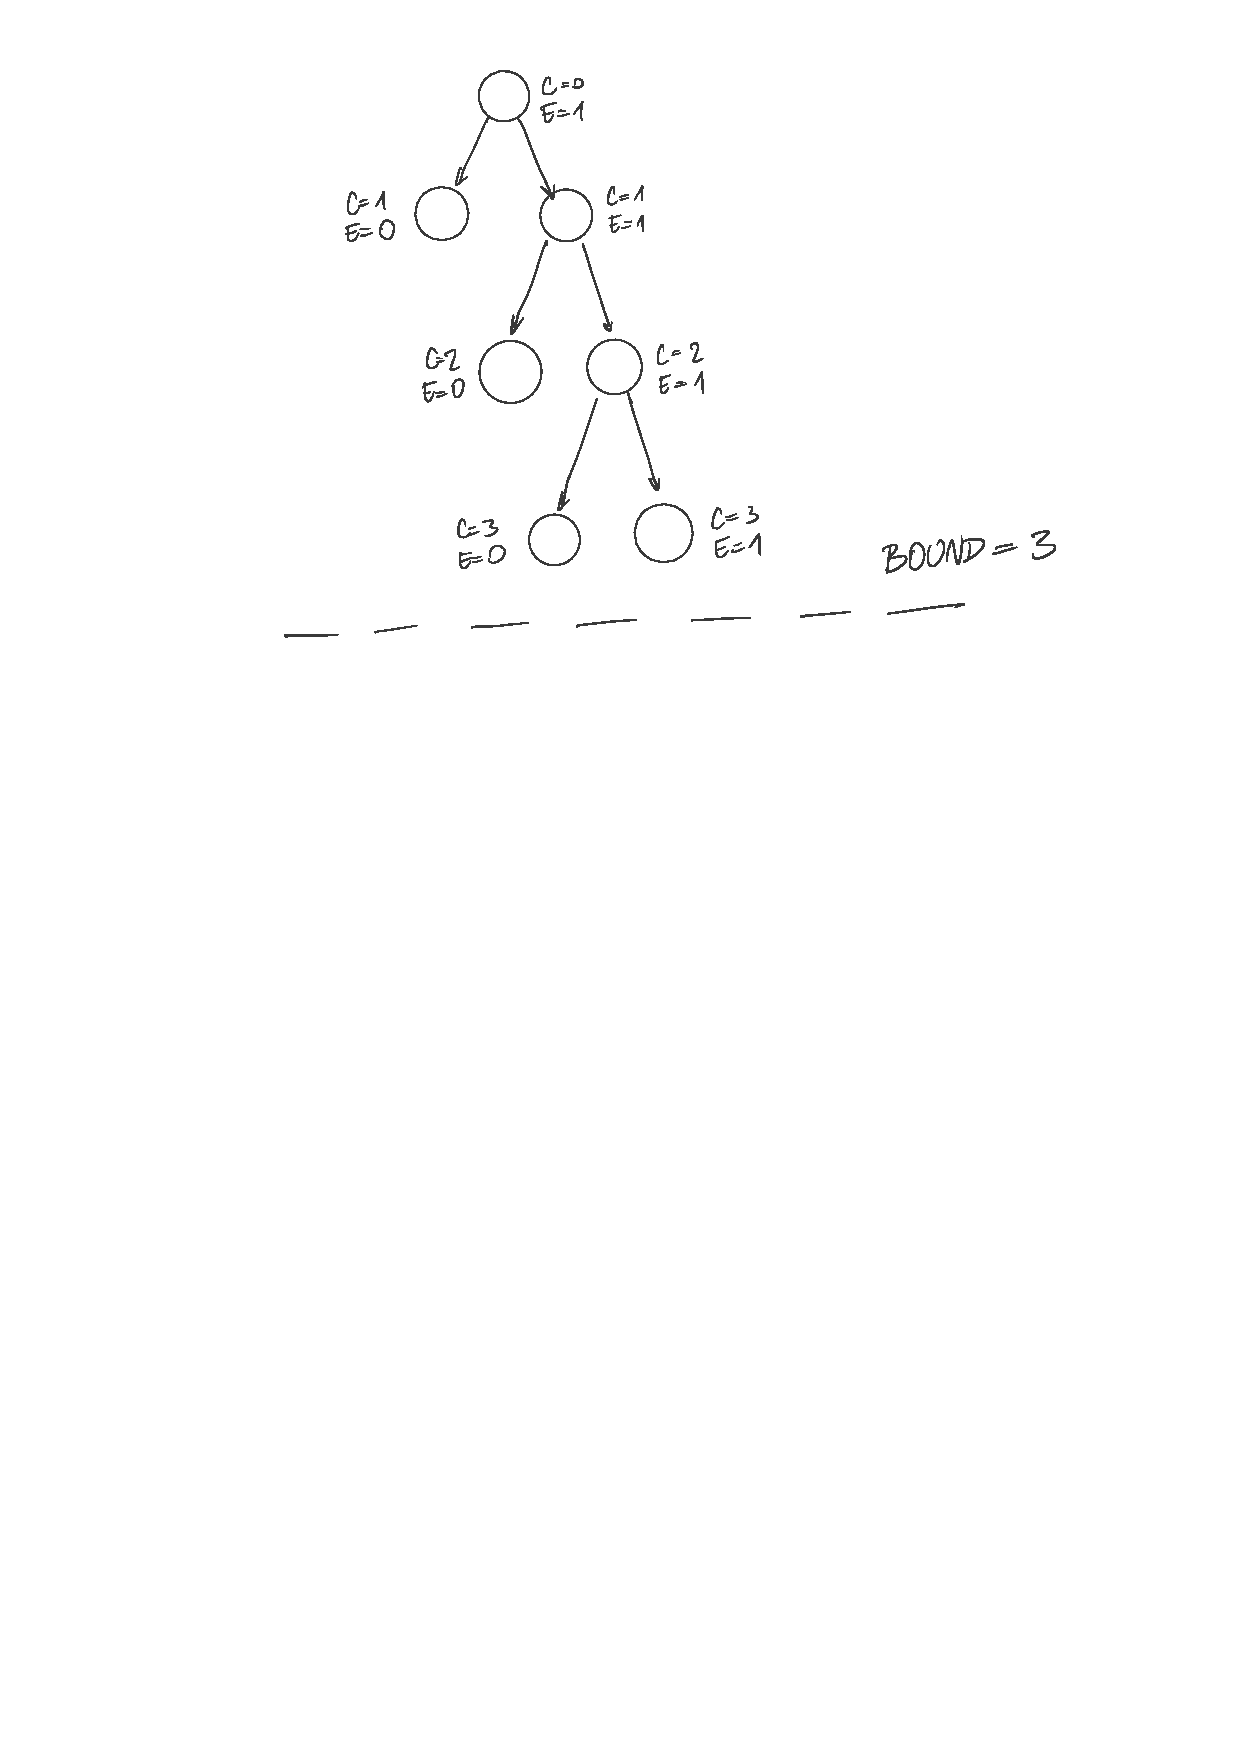
\includegraphics[scale=.6]{boundedmc}
  
\end{frame}

%%%%%%%%%%%%%%%%%%%%%%%%%%%%%%%%%%%%%%%%%%%%%%%%%%%%%%

\begin{frame}
  \frametitle{How to express properties}
 
  \begin{ntblock}
  
  \centering
In a formal language.
  \end{ntblock}
  
  \vfill

  We will use (restricted) \tc{red}{temporal logic}, which main operators are:
  \begin{itemize}
  \item \tc{blue}{always}, in every state the property holds;
  \item \tc{blue}{next}, in the next state the property holds;
  \item \tc{blue}{concatenation of $n$ next}, namely, after $n$ steps a property hold.
\end{itemize}

\vfill \pause

Full temporal logics are more expressive:
\begin{itemize}
\item \tc{blue}{until}, something must hold until something else becomes true;
\item ...
\end{itemize}

  
\end{frame}
%%%%%%%%%%%%%%%%%%%%%%%%%%%%%%%%%%%%%%%
\begin{frame}
  \frametitle{Explicit model checking (intuition)}
  
  \begin{itemize}
  \item Each formula is some sort of ``pattern''/automaton.
  
  \[ \text{E.g., } \texttt{counter}=0 \rightarrow \tc{blue}{next} \texttt{ counter}=2 \]
  
  \pause
  
  \item The algorithm checks if your model satisfies the pattern (by graph algorithms or by automata-based reasoning).
  
  \begin{center}
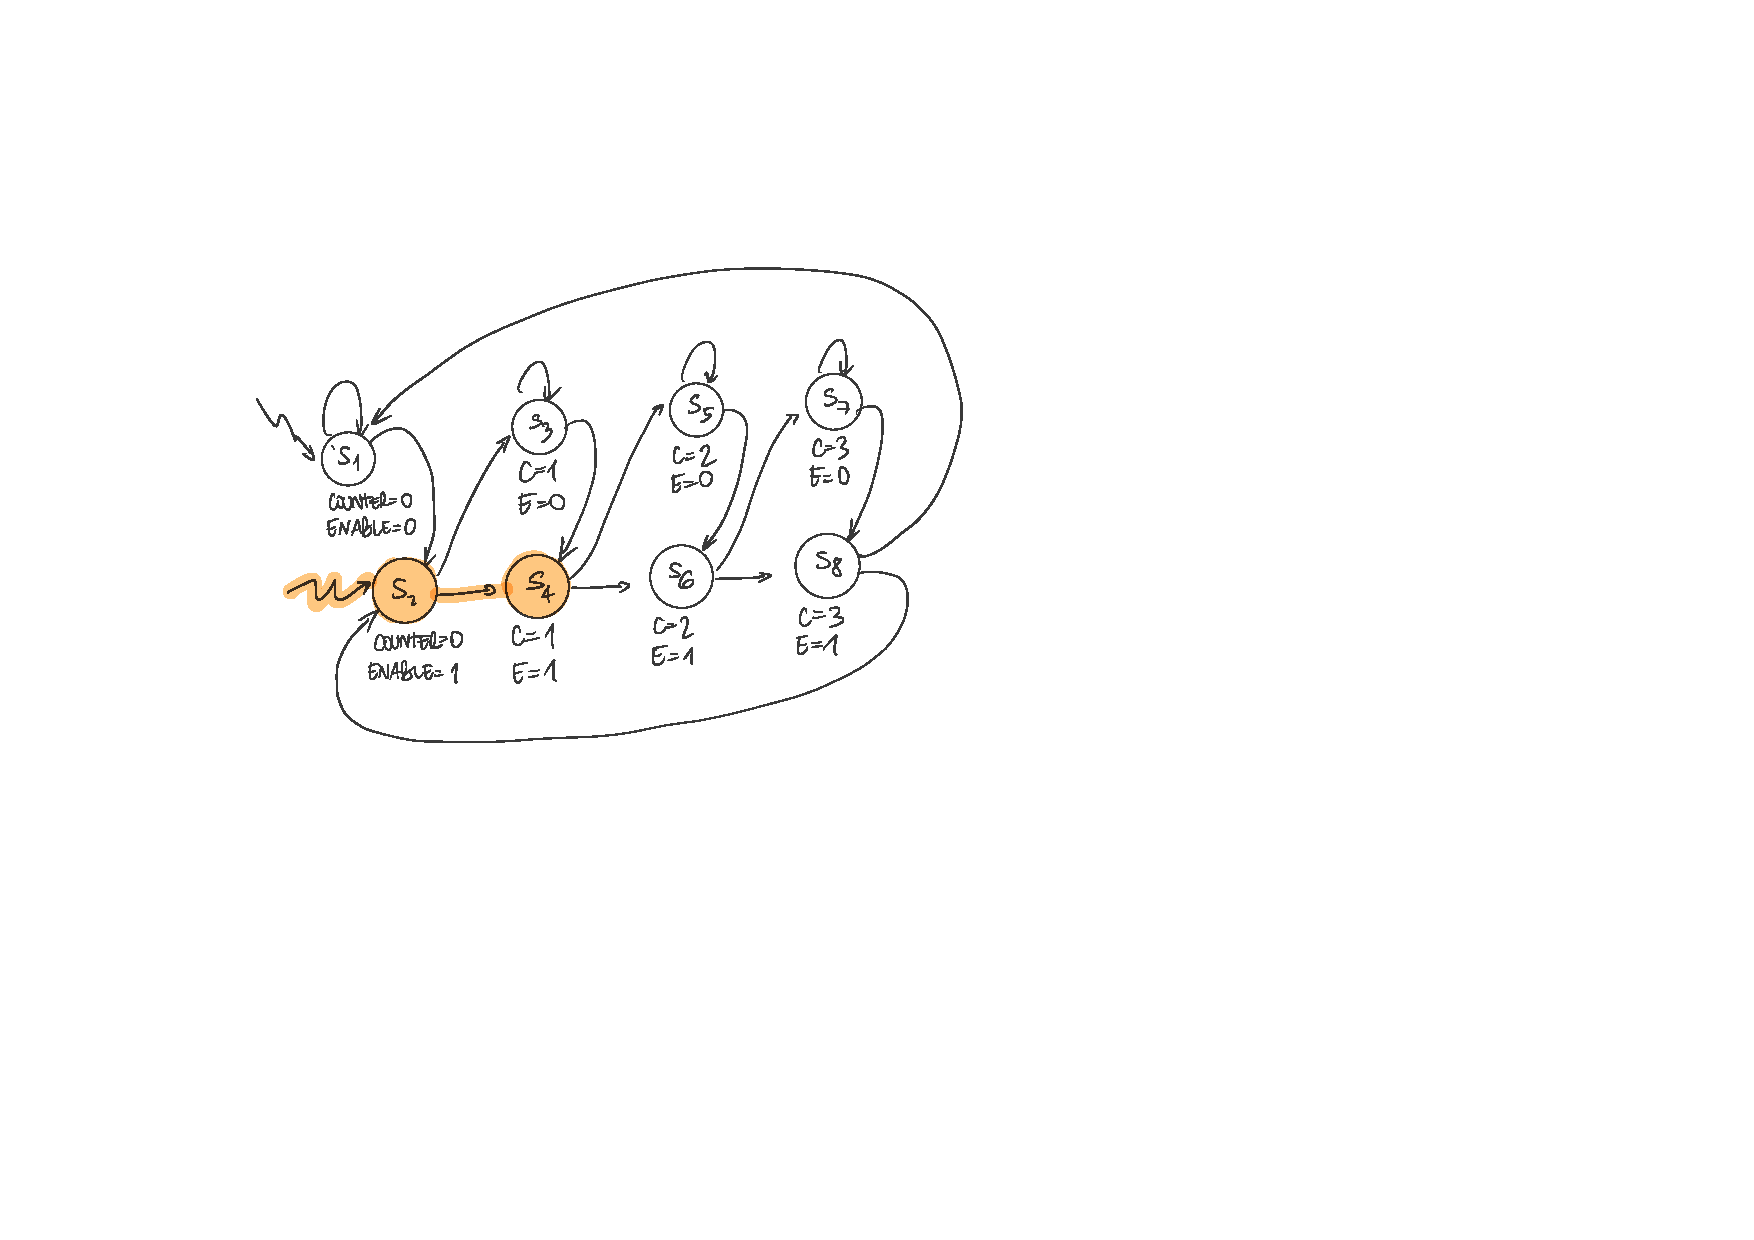
\includegraphics[scale=.3]{fsm-counter}
  \end{center}
  \pause
  \item And returns (ideally):
\begin{itemize}
  \item true if \tc{red}{all} executions satisfy the properties or
  \item false, and a \tc{orange}{counterexample} trace.
\end{itemize}

  \end{itemize}
\end{frame}

%%%%%%%%%%%%%%%%%%%%%%%%%%%%%%%%%%%
\begin{frame}
  \frametitle{Bounded model checking (intuition)}
  
\begin{minipage}[c]{0.5\textwidth}
  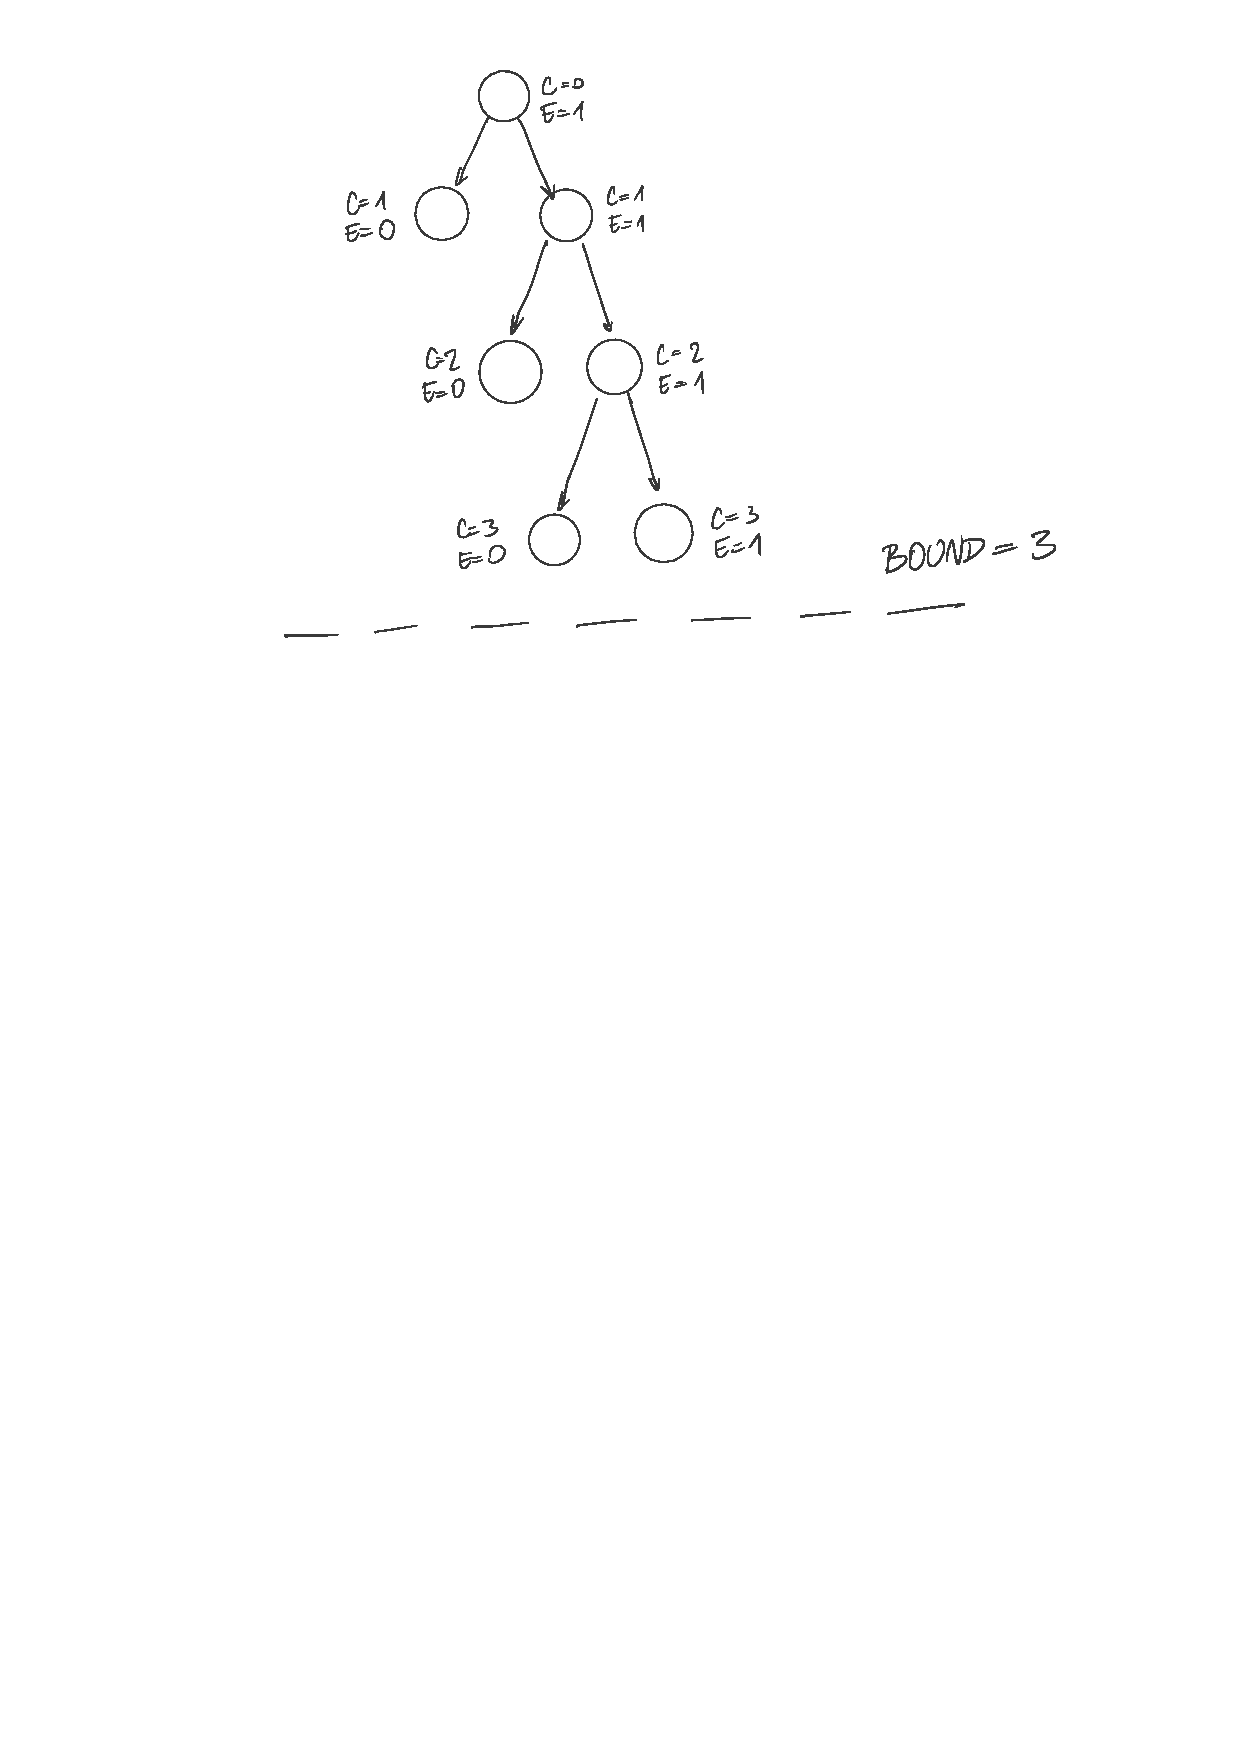
\includegraphics[scale=.3]{boundedmc}
  \end{minipage}\begin{minipage}[c]{0.5\textwidth} \begin{itemize}
  \item Relations between states is represented as a (constraint) boolean formula $R(c, e, c', e')$: 
\end{itemize}
\end{minipage}
\begin{scriptsize}
\[(c=0 \land e=1 \leftrightarrow c'=1) \land (c=0 \land e=0 \leftrightarrow c'=0) \land \ldots\]
\end{scriptsize}
\vspace{-0.3cm}
\begin{itemize} \pause
\item We unfold $R(c, e, c', e')$ a number of time equal to the bound	 (makes use of $2 \cdot 3 = 8$ variables):
\begin{scriptsize}
\[ 
\begin{array}{l}
(c_{\tc{red}{0}}=0 \land e_{\tc{red}{0}}=1 \leftrightarrow c_{\tc{red}{1}}=1) \land \ldots \\
(c_{\tc{red}{1}}=0 \land e_{\tc{red}{1}}=1 \leftrightarrow c_{\tc{red}{2}}=2) \land \ldots \\ 
\end{array} \]
\end{scriptsize}

\item we add \tc{blue}{the property} in conjunction and the \tc{blue}{initial condition}:

\begin{scriptsize}

\[ \begin{array}{l} 
 	\neg (c_{\tc{red}{0}}=0 \land c_{\tc{red}{0}}=2) \lor 
 	 	\neg (c_{\tc{red}{1}}=0 \land c_{\tc{red}{2}}=2) \lor 
 	 	 	\neg (c_{\tc{red}{2}}=0 \land c_{\tc{red}{3}}=2) \lor \ldots \land c_{\tc{red}{0}}=0
 \end{array} \]
\end{scriptsize}

\item if \tc{red}{sat}, then the property \tc{red}{does not} hold (truth assignment is the counterexample).

\end{itemize}
\end{frame}
%%%%%%%%%%%%%%%%%%%%%%%%%%%%%%%%%%%%
%%%%%%%%%%%%%%%%%%%%%%%%%%%

\begin{frame}
  \frametitle{Differences between model checking techniques}
  
 \begin{itemize}
  \item Explicit-state model checking suffers of \tc{blue}{state-explosion} problem;
  \item \tc{blue}{symbolic} model checking alleviates the problem;
  \item \tc{blue}{bounded} model checking does not verify that \tc{red}{all} executions satisfies the property, as only bounded-depth executions are checked;
  \item \tc{blue}{k-induction} use mathematical induction to prove that all executions satisfy the property (although not all properties are inductive).
\end{itemize}
  
\end{frame}





%%%%%%%%%%%%%%%%%%%%%%%%%%%%%%%%%
\section{Hands-on}
\frame{
\setbeamercovered{transparent}
\tableofcontents[currentsection,
        currentsubsection,
        subsectionstyle=shaded]
}

%%%%%%%%%%%%%%%%%%%%%%%%%%%%%%%%%%%%%%%
\begin{frame}
  \frametitle{Language we will use: \texttt{assert}}
  
  Conjunction of \tc{blue}{Always} formulas:
  \[ \texttt{assert property} (\Phi) \quad \text{where $\Phi$ can be:} \] \pause
   \begin{itemize}
  \item \tc{blue}{atomic} formula, such as: 
   \[ \texttt{unlock}, \texttt{count} < 4, ...  \]
  \item \pause \tc{blue}{boolean combination} of atomic formulas, e.g.,
  \[ \texttt{count} < 4 \; \tc{red}{\land} \; \texttt{code} \not = 3'b000  \]
  \item \pause (n-)\tc{blue}{next} formulas:
  \[ \texttt{code} \not = 3'b000 \; \tc{red}{\texttt{|=>}} \; \texttt{count} = 0 \]
    \[ \texttt{code} \not = 3'b000 \; \tc{red}{\texttt{|->} \; \#\#3} \texttt{ count} = 0 \]
\end{itemize}
\end{frame}

%%%%%%%%%%%%%%%%%%%%%%%%%%%%%%%%%%%%%%%%%%%%%%%%

\begin{frame}
  \frametitle{Language we will use: \texttt{assume}}
  
 \begin{itemize}
  \item \tc{blue}{\texttt{asserts}} are properties we want to check (for every input);
  \item \tc{blue}{\texttt{assume}} are assumptions (on the inputs).
\end{itemize}

\vfill

\begin{center}
	\texttt{assume property} \tc{red}{implies} \texttt{assert property}

\vfill \pause

\[ \begin{array}{l}
 	\texttt{assume property} (\texttt{enable} = 0) \\
\texttt{assert property} (\texttt{count |=> count})
 \end{array} \]

\end{center}
  
  
\end{frame}


%%%%%%%%%%%%%%%%%%%%%%%%%%%%%%%%%%%%%%%%%%%%%%
\begin{frame}
  \frametitle{Model checking verilog code}
  
  \begin{itemize}
  \item Time is marked by the clock (combinatorial circuits are instantaneous, as in behavioural simulation);
  \item Inputs are selected by the model checker in all possible ways;
  \item When a (or more) input(s) changes, a new ``stable'' state is computed.
\end{itemize}

  
\end{frame}



%%%%%%%%%%%%%%%%%%%%%%%%%%%%%%%%%%%%%%%%%%
\begin{frame}
  \frametitle{In practice}
  
  \begin{ntblock}
  	We will use the EBMC\footnote{\url{http://www.cprover.org/ebmc/}} model checker\footnote{\url{http://logicrunch.it.uu.se:4096/~wv/ebmc/}}. It can perform bounded model checking or incremental induction.
  \end{ntblock}

\vfill \pause

  For each module \texttt{M} we want to formally verify, we write a verification module \texttt{ReqM} which will have a set of assert properties used to verify \texttt{ReqM}.
  
  \vfill
  
In EBMC you can choose between:
\begin{itemize}
  \item bounded model checking (and set the bound);
  \item k-induction.
\end{itemize}
  
\end{frame}

%%%%%%%%%%%%%%%%%%%%%%%%%%%%%%%%%%%%%%%

\begin{frame}[fragile]
  \frametitle{Example, counter}
  
    \begin{lstlisting}[language=Verilog]
module counter(
  output [1:0] out, input enable, input clk);
...
endmodule

module counterReq(
	input enable, input clk);

 wire [1:0] out;
 counter our_count(out, enable, clk);
 
 assume property (...)
 assert property (...)
 assert property (...)  
 
 endmodule
 
 \end{lstlisting}
  
\end{frame}


%%%%%%%%%%%%%%%%%%%%%%%%%%%%%%%%%%%%%%%

\begin{frame}
  \frametitle{Suggestions}
  
  \begin{enumerate}
  \item Most properties relate past values with new values: use registers in the \texttt{Req} module to save the past values.
	  \item \tc{red}{Avoid latches at all costs} in the design!
  \end{enumerate}

  
\end{frame}



%%%%%%%%%%%%%%%%%%%%%%%%%%%%%%%%%%%%%%%


%%%%%%%%%%%%%%%%%%%%%%%%%%%%%%%%%%%%%%%



%%%%%%%%%%%%%%%%%%%%%%%%%%%%%%%%%%%%%%%




%%%%%%%%%%%%%%%%%%%%%%%%%%%%%%%%%%%%%%%




%%%%%%%%%%%%%%%%%%%%%%%%%%%%%%%%%%%%%%%



%%%%%%%%%%%%%%%%%%%%%%%%%%%%%%%%%%%%%%%




%%%%%%%%%%%%%%%%%%%%%%%%%%%%%%%%%%%%%%%

\end{document}